
%(BEGIN_QUESTION)
% Copyright 2011, Tony R. Kuphaldt, released under the Creative Commons Attribution License (v 1.0)
% This means you may do almost anything with this work of mine, so long as you give me proper credit

It is common practice to connect an antenna to a radio transceiver (transmitter/receiver) using a transmission line if the antenna must be located somewhere high up for good reception.  In this particular example, a radio transceiver is used to communicate natural gas flow measurement data from a flow computer to some far-away location, as part of a SCADA system for the natural gas pipeline.  The antenna is located at the top of a wooden pole for better signal strength than if it were located at ground level:

$$\includegraphics[width=15.5cm]{i01357x01.eps}$$

In this installation, the transmission line is a 20 foot length of 50 $\Omega$ coaxial cable.  Knowing that reflected signals are bad in any transmission line system, the technician who installed this system also installed a 50 $\Omega$ {\it termination resistor} at the antenna-end of the cable, in parallel with the antenna.

Was the installation of this termination a good idea, or not?  Explain your answer.

\vskip 20pt \vbox{\hrule \hbox{\strut \vrule{} {\bf Suggestions for Socratic discussion} \vrule} \hrule}

\begin{itemize}
\item{} Explain how a TDR could be used to check the transmission line for proper termination.
\item{} For those who have studied gas flow measurement, what does {\it AGA3} mean, and why are there {\it three} process transmitters connected to the flow computer?
\item{} Explain what a ``SCADA'' system is and what function it fulfills.
\item{} It is quite common to find analog transmitters in solar-powered SCADA monitoring sites using {\it voltage} signal ranges rather than the {\it current} signals more commonly found in industrial (plant) applications.  The reason for this is to reduce power consumption.  Explain how the use of voltage signaling reduces power consumption compared to current signaling.
\item{} Is this a true example of a ``SCADA'' node, or might it best be characterized as a {\it telemetry} node?  Explain your answer.
\end{itemize}

\underbar{file i01357}
%(END_QUESTION)





%(BEGIN_ANSWER)

There is absolutely no need for a termination resistor at the end of a transmission line terminating in an antenna.

%(END_ANSWER)





%(BEGIN_NOTES)

Don't put a terminator on the cable, because that would absorb the signal pulses!  Instead, you want the antenna itself to act as the dissipating element.  If the antenna is properly matched to the cable, it will adequately terminate the cable for minimum signal reflections within the cable because the antenna will act as a dissipative load.

%INDEX% Electronics review: antennas
%INDEX% Electronics review: characteristic impedance of transmission line
%INDEX% Electronics review: surge impedance of transmission line

%(END_NOTES)


